\chapter{A detailed derivation of the \textit{one-fluid}, \textit{two-fluid} and volume averaged formulation of a generalized balance equations.}
\label{ap:average}

\section{General balance equations}

\begin{figure}[h]
    \centering
    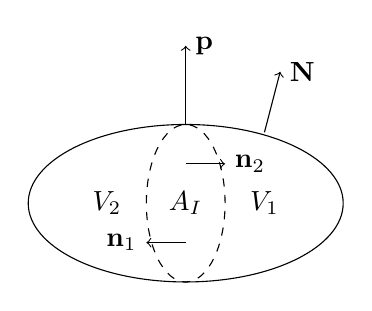
\begin{tikzpicture}
        \draw (0,0) ellipse (2 and 1);
        \draw[dashed] (0,0) ellipse (0.5 and 1)node{$A_I$};
        \draw[->](0,1)--++(0,1)node[right]{\textbf{p}}; 
        \draw[->](1,0.9)--++(0.2,0.77)node[right]{\textbf{N}}; 
        \draw[->](0,-0.5)--++(-0.5,0)node[left]{$\textbf{n}_1$}; 
        \draw[->](0,0.5)--++(0.5,0)node[right]{$\textbf{n}_2$}; 
        \draw (1,0)node{$V_1$};
        \draw (-1,0)node{$V_2$};
    \end{tikzpicture}
    \caption{Scheme of an arbitrary material control volume.   }
\end{figure}

Let $f^0$  be an arbitrary quantity to be conserved inside the non-material volume $\omega$. 
Then $\bm\Phi^0$ refer to the non-convective flux of $f^0$. 
Then $s^0$ refer to source term  related to  $f^0$. 
Then, for an arbitrary control volume we have, 
\begin{equation*}
    \ddt \int_{V} f^0 dV 
    = 
    \int_{V} s^0 dV 
    + \int_{\partial V} \mathbf{\Phi}^0 \cdot \textbf{N} dS,
\end{equation*}
where $\textbf{N}$ is the normal of the control volume. 
Any quantities defined in $V_k$ will be noted with a subscript $_k$ and those who are defined at the interface with $_I$. 
Therefore, if we decompose any quantity such as $f^0 = \sum_k f_k^0 \chi_k + f_I^0 \delta_I$ we obtain, 
\begin{multline*}
    \sum_k\left[\ddt \int_{V_k} f_k^0 dV 
    - \int_{V_k} s_k^0 dV 
    - \int_{A_k} \mathbf{\Phi}_k^0 \cdot \textbf{N} dS
    \right]
    + \ddt \int_{A_I} f_I^0 dS 
    - \int_{A_I} s_I^0 dS 
    - \int_{C} \mathbf{\Phi}_I^0 \cdot \textbf{p} dC 
    = 0
\end{multline*}
Using the Reynolds transport theorem on volume integral yields,
\begin{align*}
    \ddt \int_{V_k} f_k^0 dV 
    &= \int_{V_k} \pddt f_k^0 dV 
    + \int_{A_I \cup A_k} f_k^0 \textbf{u} \cdot \textbf{n}_k dS\\
    &= \int_{V_k} \left[
        \pddt f_k^0  + \div (f_k^0 \textbf{u}_k^0) 
    \right]dV 
    + \int_{A_I} f_k^0 (\textbf{u}_I^0 - \textbf{u}_k^0) \cdot \textbf{n}_k dS\\
\end{align*}
where $\textbf{n}_k$ is the normal of the interface $A_I$ on the outward direction of the $k$ phase. 

The second term is integrated only over $A_I$ as it is the interface between both phase and not the one of the control volume. 
Using the Ledbiz rule for integration on surface yields, 
\begin{align*}
    \ddt \int_{A_I} f_I^0 dS 
    &= \int_{A_I} \left[
        \pddt f_I^0  + \divI (f_I^0 \textbf{u}_I^0) 
    \right]dS
\end{align*}

Regarding the non-convective integrals, by using the divergence theorem we can write\citep{nadim1996concise}, 
\begin{align*}
    \int_{A_k} \mathbf{\Phi}_k^0\cdot \textbf{n}_k dS
    = \int_{V_k} \div\mathbf{\Phi}_k^0 dV
    - \int_{A_I} \mathbf{\Phi}_k^0\cdot \textbf{n}_k dS. 
\end{align*}
The last term can also be re-written with the divergence theorem \citet{nadim1996concise},
\begin{align*}
    \int_{C} \mathbf{\Phi}_I^0\cdot \textbf{p} dC 
    = \int_{A_I} \divI \mathbf{\Phi}_I^0 dS
    - \int_{A_I} \mathbf{\Phi}_I^0 \cdot \textbf{n} \div \textbf{n} dS
\end{align*}
Notice that whether it is $\textbf{n}_1$ or $\textbf{n}_2$ the second term on the left conserve the same sign. 

Taking in account these reformulations, we can re-write the integral balance previously exposed by, 
\begin{align*}
    \sum_k \int_{V_k}{\left[
        \pddt f_k^0
        + \div (f_k^0\textbf{u}_k^0 - \bm\Phi_k^0)
        - s_k^0
    \right]}\\
    + \sum_k\int_{A_I}{\left[
        f_k^0(\textbf{u}_I^0 - \textbf{u}_k^0)
        + \bm\Phi_k^0
    \right]\cdot \textbf{n}_k}
    + \int_{A_I}{\left[
        \pddt f_I^0 
        + \divI (f_I^0 \textbf{u}_I - \bm\Phi_I^0)
        + \bm\Phi_I^0 \cdot \textbf{n} \div \textbf{n}
    \right]} =0 
\end{align*}

Every integral of volume must be balanced independently of the surface integral. 
This means that we can separate this equation into two, 
\begin{equation*}
    \pddt f_k  
    + \div (f_k \textbf{u}_k - \mathbf{\Phi}_k) 
    =s_k. 
\end{equation*}
\begin{equation}
    \pddt f_I  
    + \divI (f_I \textbf{u}_I -\mathbf{\Phi}_I)
    + \mathbf{\Phi}_I \cdot \textbf{n} \div \textbf{n}
    = 
    + s_I
    - \sum_k \left[
    f_k (\textbf{u}_I - \textbf{u}_k)
    + \mathbf{\Phi}_k
    \right] \cdot \textbf{n}_k. 
    \label{ap:eq:dt_f_I}
\end{equation}
These equations are valid in $\Omega_k(t)$ and $\Sigma(t)$ for volume and surface quantity, respectively. 

Now let's reformulate the third term of the surface balance equation. 
Let $\textbf{F}$ be an arbitrary surface quantity. 
It can be split into two part such as, 
\begin{equation*}
    \textbf{F} 
    = \textbf{F} \cdot \textbf{n}\textbf{n}
    + (\textbf{I} - \textbf{nn})  \cdot \textbf{F}
    = \textbf{F}_\bot + \textbf{F}_{||}.
\end{equation*}
Injecting this decomposition inside the Gauss theorem on an arbitrary control volume it can be shown that, 
\begin{equation*}
    \int_{S} \divI \textbf{F}dS
    = 
    \int_{S} \left[\divI \textbf{F}_{||} 
    + \textbf{F} \cdot \textbf{n} \div\textbf{n}
    \right]dS
\end{equation*}
Consequently, we have the following relation,
\begin{equation*}
    \int_{A_I} \divI \bm\Phi_I^0dS
    = 
    \int_{A_I} \left[\divI \bm\Phi_{I||}^0
    + \bm\Phi_I^0 \cdot \textbf{n} \div\textbf{n}
    \right]dS
\end{equation*}

By taking in account this relation it is easy to take or not the normal components of a vector to the interface within the balance equaitons. 
For example, we can write either, 
\begin{equation}
    \pddt f_I  
    + \divI (f_I \textbf{u}^I_{||} -\mathbf{\Phi}^I_{||})
    + f_I \textbf{u}_I \cdot \textbf{n} \div \textbf{n}
    - s_I
    = 
    - \sum_k \left[
    f_k (\textbf{u}_I - \textbf{u}_k)
    + \mathbf{\Phi}_k
    \right] \cdot \textbf{n}_k 
    \label{ap:eq:dt_f_I2}
\end{equation}
Or 
\begin{equation}
    \pddt f_I  
    + \divI (f_I \textbf{u}^I -\mathbf{\Phi}^I_{||})
    - s_I
    = 
    - \sum_k \left[
    f_k (\textbf{u}_I - \textbf{u}_k)
    + \mathbf{\Phi}_k
    \right] \cdot \textbf{n}_k 
    \label{ap:eq:dt_f_I2}
\end{equation}
where we have changed the flux term formulation. 



\section{Topological equations}
There is two Topological equaitons one for $\chi_k$ and an other for $\delta_I$.
First, we recall the relations related to the phase indicator function, 
\begin{equation}
    \frac{\partial}{\partial t} \chi_k
    + \textbf{u}_I  \grad \chi_k 
    = 0, \;\;\;\;\text{and}\;\;\;\; 
    \grad \chi_k 
    = - \delta_I \textbf{n}_k.
    \label{ap:eq:phase_properties}
\end{equation}
Now the surface indicator function transport equation can be obtained using the Leibniz rule for differentiation,  
\begin{equation*}
    \ddt \int_{A_I} dS
    = \int_{A_I} \grad_I \cdot \textbf{u}_I dS,
\end{equation*}
Those integrals can be re rewritten as, 
\begin{equation*}
    \ddt \int_{V} \delta_I dV
    = \int_{V} \delta_I \grad_I \cdot \textbf{u}_I dV.
\end{equation*}
Then using the Reynolds transport term for fixed material volume yields,
\begin{equation*}
    \pddt \delta_I
    + \grad \cdot (\delta_I \textbf{u}_I)
    = \delta_I \grad_I \cdot \textbf{u}_I. 
\end{equation*}
This equation can also be takes the form 
\begin{equation}
    \pddt \delta_I
    + \grad \cdot (\delta_I \textbf{u}_I\cdot \textbf{n}\textbf{n})
    = \delta_I \textbf{u}_I \cdot \textbf{n}\grad \cdot \textbf{n}. 
    \label{ap:eq:dt_delta_I}
\end{equation}
Also, it can be useful to derive an expression for the gradient of the $\delta_I$ function. 
To do so we take the gradient of \ref{ap:eq:phase_properties} yielding, 
\begin{equation*}
    \grad\delta_I 
    = \grad( - \textbf{n}_k \cdot \grad \chi_k)
    = \grad\textbf{n}_k \cdot \textbf{n}_k \delta_I
    + \grad(\textbf{n}_k \delta_I) \cdot \textbf{n}_k 
\end{equation*}
Note that the first term on the LHS vanish

\section{\textit{One-fluid} and \textit{two-fluid} formulations}
In this appendix we derive the \textit{two-fluid} and \textit{one-fluid} formulation of a generalized conservation equation, namely,
\begin{equation}
    \frac{\partial}{\partial t} f_k
    = \grad \cdot (\bm{\Phi}_k - f_k\textbf{u}_k)
    + \textbf{S}_k.
    \label{ap:eq:global_balance}
\end{equation}
Then we derive the phase averaged and global averaged equation of this general equation of conservation. 

We can derive the \textit{two-fluid} formulation by multiplying \ref{ap:eq:global_balance} by the phase indicator function \ref{eq:phase_indicator}. 
It yields, 
\begin{equation*}
    \frac{\partial}{\partial t} (\chi_k f_k)
    = \grad \cdot (\chi_k \bm{\Phi}_k - \chi_k f_k \textbf{u}_k)
    + \chi_k \textbf{S}_k.
    + f_k \frac{\partial}{\partial t} \chi_k
    + \left(
        f_k \textbf{u}_k 
        - \bm{\Phi}_k
    \right) \cdot \grad \chi_k
    % \label{ap:eq:global_balance}
\end{equation*}
where we have included the phase function $\chi_k$ into the derivative operators. 
Now, using the \ref{ap:eq:phase_properties} we get, 
\begin{equation}
    \frac{\partial}{\partial t} (\chi_k f_k)
    = \grad \cdot (\chi_k \bm{\Phi}_k - \chi_k f_k \textbf{u}_k)
    + \chi_k \textbf{S}_k
    + \left[
        \bm{\Phi}_k 
        + f_k 
        \left(
            \textbf{u}_I
            - \textbf{u}_k
        \right) 
    \right]
    \cdot \textbf{n}_k \delta_I 
    \label{ap:eq:two-fluid_global}
\end{equation}
where the last term is the interfacial source term, such as the drag force if $f_k$ is the momentum or the mass transfer if $f_k$ is the density. 
In this equation notice that all quantities are factor of the phase indicator function $\chi_k$. 
So we transport $\chi_k f_k$ which is field quantity defined over the whole domain. 
Thus, \ref{ap:eq:two-fluid_global} is valid over the entire domain.   

Now, we define the jump condition across the interface or the surface transport equation as the sum of the interfacial term on each phase $k$. 
It can be obtained using  the transport of surface \ref{ap:eq:dt_f_I2}.
Indeed, multiplying \ref{ap:eq:dt_f_I2} by $\delta_I$ gives, 
\begin{equation}
    \pddt (f_I\delta_I)  
    = 
    + \grad \cdot (\delta_I \mathbf{\Phi}^I_{||} - \delta_I f_I \textbf{u}^I)
    +\textbf{S}_I \delta_I
    - \sum_k \left[
    f_k (\textbf{u}_I - \textbf{u}_k)
    + \mathbf{\Phi}_k
    \right] \cdot \textbf{n}_k \delta_I
    \label{ap:eq:general_jump}
\end{equation}
\tb{
    Notice that the first term on the RHS is the parallele component of $\mathbf{\Phi}$ thus it must be reformulated as, 
    
}

Now, let's derive the \textit{one-fluid} formulation of the general conservation law.
To do so we sum on all phases \ref{ap:eq:two-fluid_global} plus the interface. 
Besides, we define any quantities $q$ such as, $q = \sum_k \chi_k q_k + \delta_I q_I$.
Then it is trivial to show that, 
\begin{equation}
    \frac{\partial}{\partial t} f
    = \grad \cdot (\bm{\Phi} - f \textbf{u})
    + \textbf{S}
    \label{ap:eq:one-fluid_global}
\end{equation}
which is the \textit{one-fluid} formulation. 

The volume average of \ref{ap:eq:two-fluid_global} is then straight forward, by using the definition of the averaged operator, we get, 
\begin{equation*}
    \frac{\partial}{\partial t} (\phi_k\kavg{f})
    = \grad \cdot \left(
        \phi_k \kavg{\bm{\Phi} - f \textbf{u}}
    \right)
    + \phi_k \kavg{\textbf{S}}
    + a_I \Iavg{
        \bm{\Phi}_k \cdot \textbf{n}_k
        + f_k 
        \left(
            \textbf{u}_I
            - \textbf{u}_k
        \right) \cdot \textbf{n}_k
    } 
\end{equation*}
Similarly, the bulk average can be obtained by averaging \ref{ap:eq:one-fluid_global} yielding, 
\begin{equation*}
    \frac{\partial}{\partial t} \avg{f}
    = \grad \cdot \avg{\bm{\Phi} - f \textbf{u}}
    + \avg{\textbf{S}}
    % + a_I\avg{\textbf{J}_I},
    \label{ap:eq:avg_global}
\end{equation*}
\section{Derivation of the point velocity}
Consider a particle of center of mass $\textbf{y}_\alpha$ defined such as
\begin{equation*}
    m_\alpha \textbf{y}_\alpha
    = \int_{V_\alpha} \rho_k \textbf{y}_k dV,
\end{equation*}
its velocity can be solely the derivation of $\textbf{y}_\alpha$ whitin time.
Yielding, 
\begin{align*}
    \ddt \textbf{y}_\alpha (t)
    &=
    \ddt \left(
        \frac{1}{m_\alpha} \int_{V_\alpha} \rho_k \textbf{y}_k dV
    \right)\\
    &= \frac{1}{m_\alpha}
    \ddt 
    \left(
        \int_{V_\alpha} \rho_k \textbf{y} dV
    \right)
    - \frac{1}{m_\alpha^2} \ddt \int_{V_\alpha} \rho_k dV \int_{V_\alpha} \rho_k \textbf{y}_k dV
    \\
    &= \frac{1}{m_\alpha}\int_{V_\alpha} \left[
        \pddt (\rho_k \textbf{y}) + \grad \cdot\left(\rho_k \textbf{y}\textbf{u}_k\right) dV 
    \right]\\
    &+ \frac{1}{m_\alpha}\int_{S_\alpha} \textbf{y} M_k d S
    -  \frac{1}{m_\alpha^2} \int_{S_\alpha} M_k dS  \int_{V_\alpha} \rho_k \textbf{y}_k dV
    \\
    &= \frac{1}{m_\alpha}\int_{V_\alpha} \textbf{y} \left[
    \pddt (\rho_k) + \grad \cdot\left(\rho_k \textbf{u}_k\right) dV 
    \right]dV
    + \frac{1}{m_\alpha}\int_{V_\alpha} \rho_k  \textbf{u}_k  \cdot \grad \textbf{y} dV \\
    &+ \frac{1}{m_\alpha}\int_{S_\alpha} \textbf{y}_k M_k d S
    - \frac{1}{m_\alpha}  \textbf{y}_\alpha \int_{S_\alpha} M_k dS
\end{align*}
By considering the mass conservation \ref{eq:single-fluid_mass} for the first term,  noticing that $\grad \textbf{y} = \textbf{I}$ where $\textbf{I}$ is the identity tensor for the second term and introducing \textbf{r} in the third term gives, we get the following relation,
\begin{equation*}
    \textbf{u}_\alpha
    = \frac{1}{m_\alpha} \left(
        \textbf{p}_\alpha
        +  \int_{S_\alpha} \textbf{r} M_k dS
    \right)
    % = \frac{1}{m_\alpha}  \left(
    %     \textbf{p}_\alpha
    % - \int_{V_\alpha} \rho_k \textbf{w} dV
    % \right)
\end{equation*}

\section{Derivation of the surface transport equations for Lagrangian particles}

By making use of the Leibniz rule together with \ref{ap:eq:dt_f_I} it can be shown that for any surface quantity $f_I$ we have, 
\begin{align*}
    \ddt \int_{S_\alpha} f_I dS
    &= \int_{S_\alpha} \pddt f_I 
    + \grad_I \cdot (\textbf{u}_If_I) dS\\
    &= \int_{S_\alpha} \left(
        \grad_I \cdot \mathbf{\Phi}_{||}^I
        + \textbf{S}_I
    \right) dS\\
    & - \sum_k \int_{S_\alpha} \left[
        f_k (\textbf{u}_I - \textbf{u}_k)
        + \mathbf{\Phi}_k
    \right] \cdot \textbf{n}_k
    dS
\end{align*}
Then remark that if $\mathbf{\Phi} = \sigma (\textbf{I}-\textbf{nn})$.
Then, 
\begin{equation*}
    \int_S \grad_I \cdot \left[\sigma (\textbf{I} - \textbf{nn})\right]dS 
    =
    \int_S  \grad_I \sigma dS 
    + \int_S \sigma \kappa \textbf{n}dS 
    = 0
\end{equation*}

Using the Gauss theorem for closed surface it can be shown easily that the first term on the RHS can be reformulated, leaving with, 
\begin{align}
    \ddt \int_{S_\alpha} f_I dS
    = \int_{S_\alpha} \left[
        \textbf{S}_I 
        - \kappa \mathbf{\Phi}_{||}^I\cdot \textbf{n} 
    \right]dS
    - \sum_k \int_{S_\alpha} \left[
        f_k (\textbf{u}_I - \textbf{u}_k)
        + \mathbf{\Phi}_k
    \right] \cdot \textbf{n}_k
    dS
\end{align}
In this equation we can see that $\mathbf{\Phi}_I$ plays no role at all. 

Now let's derive the first moment of a surface quantity, namely $f_I \textbf{r}$. 
\begin{align*}
    \ddt \int_{S_\alpha} f_I \textbf{r} dS
    &= \int_{S_\alpha} \textbf{r}\left[
        \pddt f_I 
        + \grad_I \cdot (\textbf{u}_If_I) 
    \right]dS
    + \int_{S_\alpha}
    f_I \left[
        \pddt \textbf{r} + \textbf{u}_I \cdot \grad_I \textbf{r}
    \right]
    dS\\
\end{align*}
Using \ref{ap:eq:dt_f_I} on the first term of the RHS and the relation $\grad_I \textbf{r} = (\textbf{I} - \textbf{nn})$ gives, 
\begin{align*}
    \ddt \int_{S_\alpha} f_I \textbf{r} dS
    &= \int_{S_\alpha} \textbf{r}\left[
        \grad_I \cdot \mathbf{\Phi}_I
        - \Phi_I\cdot\textbf{n}\grad\textbf{n}
        + \textbf{S}_I
    \right] dS\\
    & - \sum_k \int_{S_\alpha}\textbf{r} \left[
        f_k (\textbf{u}_I - \textbf{u}_k)
        + \mathbf{\Phi}_k
    \right] \cdot \textbf{n}_k
    dS\\
    &+ \int_{S_\alpha}
    f_I (\textbf{u}^I_{||} - \textbf{u}_\alpha)
    dS\\
\end{align*}
Using the Gauss theorem for closed surface on the first term on the RHS, this equation can be simplified to, 
\begin{align}
    \ddt \int_{S_\alpha} f_I \textbf{r} dS
    &= \int_{S_\alpha} \left(
        \textbf{S}_I\textbf{r}
        - \mathbf{\Phi}_{||}^I
    \right) dS
    + \int_{S_\alpha}
    f_I \textbf{w}_I
    dS\nonumber\\
    & - \sum_k \int_{S_\alpha}\textbf{r} \left[
        f_k (\textbf{u}_I - \textbf{u}_k)
        + \mathbf{\Phi}_k
    \right] \cdot \textbf{n}_k
    dS
    \label{ap:eq:dt_r_f_I}
\end{align}
where $\textbf{w}_{I||} = \textbf{u}_{I||} - \textbf{u}_\alpha$. 
In the jump condition of the first moment it is now evident that $\mathbf{\Phi}^I_{||}$ is relevant. 

As an example, if $f_I$ were to be the momentum of the surface, then $\mathbf{\Phi}_{||}^I = \sigma (\textbf{I} - \textbf{nn})$. 
Thus, we can express the integrals as, 
\begin{equation*}
    \int_{S_\alpha}\mathbf{\Phi}_{||}^IdS
    =\int_{S_\alpha} \sigma (\textbf{I} - \textbf{nn}) dS
    =\int_{S_\alpha} \grad_I \cdot (\sigma \textbf{r}) dS
    =\int_{S_\alpha} \sigma \textbf{r} (\grad\cdot\textbf{n}) \textbf{n} dS
\end{equation*} 
where we used the Gauss theorem on closed surface for the first term. 
In this last expression we recognize the last term as begin the first moment of the surface tension force. 




\section{Decomposition of the particular energy balance.}
This section is a detailed derivation of the energy equation for a whole fluid particle, namely,
\begin{equation*}
    \label{ap:eq:E_alpha_dt}
    \ddt E_\alpha 
    % = \ddt \int_{V_\alpha} \rho_k E_k dV
    = \int_{V_\alpha} \textbf{b}_k \cdot \textbf{u}_k dV
    + \int_{S_\alpha} \left[
        (\textbf{T}\cdot \textbf{u} 
    - \textbf{q})\cdot\textbf{n}_k 
    + M_k E_k 
    + \textbf{f}_I \cdot \textbf{u}_I 
    \right]dS, 
\end{equation*}
Since we can decompose the velocity fields of a particle following $\textbf{u}_k = \textbf{u}_\alpha + \textbf{w}$ it is then possible to rewrite the total energy, 
Yielding, 
\begin{multline*}
    \int_{V_\alpha} \rho_k E_k dV
    = \int_{V_\alpha} \rho_k e_k dV
    + \frac{1}{2} \int_{V_\alpha} \rho_k \textbf{u}_\alpha\cdot\textbf{u}_\alpha dV\\
    + \int_{V_\alpha} \rho_k \textbf{u}_\alpha\cdot\textbf{w} dV
    + \frac{1}{2} \int_{V_\alpha} \rho_k \textbf{w}\cdot\textbf{w} dV
\end{multline*}
by applying the relation \ref{eq:M_alpha_dt} on the second term, it is possible to show that,
\begin{equation*}
    E_\alpha
    = \int_{V_\alpha} \rho_k e_k dV
    + \frac{1}{2} \textbf{u}_\alpha\cdot\textbf{u}_\alpha  m_\alpha
    + \textbf{u}_\alpha\cdot \int_{V_\alpha} \rho_k \textbf{w} dV
    + \frac{1}{2} \int_{V_\alpha} \rho_k \textbf{w}\cdot\textbf{w} dV.
\end{equation*}
We clearly see that the energy can be decomposed into internal and kinetic energy. 
We define the integrated internal energy of the particle by $e_\alpha = \int_{V_\alpha} = \rho_k e_k dV$.
It is the straight forward (using \ref{eq:one-fuild_internal_energy}) to show that, 
\begin{equation*}
    \ddt e_\alpha
    = \int_{V_\alpha} \textbf{T}:\grad\textbf{u}_k dV
    + \int_{S_\alpha} \left(
        e_k M_k
        - \textbf{q}_k \cdot \textbf{n}_k
    \right) dS.
\end{equation*}
Similarly, the kinetic energy equation for a whole fluid particle can be obtained deriving the local kinetic energy ,namely,
\begin{equation*}
    \ddt \int_{V_\alpha} \rho_k \frac{u_k^2}{2} dV
    = \int_{V_\alpha}\textbf{u}_k \cdot  \left(
        \textbf{b}_k
        + \grad \cdot \textbf{T}_k
    \right)dV
    + \int_{S_\alpha} \frac{u_k^2}{2} M_k dS.
\end{equation*}
Using the velocity decomposition one can deduce, 
\begin{multline}
    \frac{1}{2} \ddt \left(
        m_\alpha \textbf{u}_\alpha \cdot \textbf{u}_\alpha
        + 2\textbf{u}_\alpha \cdot \int_{V_\alpha}  \rho_k \textbf{w}_k dV
        + \int_{V_\alpha} \rho_k \textbf{w}_k \cdot \textbf{w}_k dV
    \right)\\
    =  \textbf{u}_\alpha \left[
        \cdot\int_{V_\alpha} \textbf{b}_k dV
        +  \int_{S_\alpha} \left(
            \textbf{T}_k \cdot \textbf{n}_k
            + \frac{1}{2} \textbf{u}_\alpha M_k 
            + \textbf{w}_k M_k 
        \right)dS
    \right]\\
    + \int_{V_\alpha} \left(
        \textbf{w}_k\cdot\textbf{b}_k
        -\textbf{T}_k : \grad \textbf{w}_k
    \right)dV
    + \int_{S_\alpha} 
        \textbf{w}_k\cdot(\textbf{T}_k\cdot \textbf{n}_k)
    dS\\
    + \int_{S_\alpha} \frac{1}{2} \textbf{w}_k \cdot \textbf{w}_k M_k dS.
    \label{ap:eq:u_2_dt}
\end{multline}
Besides, taking the dot product of the centered velocity $\textbf{u}_\alpha$, with the momentum equation \ref{eq:dt_p_alpha}, gives, 
\begin{multline*}
    \frac{1}{2}\ddt (m_\alpha \textbf{u}_\alpha \cdot \textbf{u}_\alpha)
    + \textbf{u}_\alpha \cdot \ddt \int_{V_\alpha} \rho_k \textbf{w}_k dV \\
    = \textbf{u}_\alpha \cdot \int_{V_\alpha} \textbf{b}_k dV
    + \textbf{u}_\alpha \cdot \int_{S_\alpha} \left(
    \textbf{T}_k \cdot\textbf{n}_k
    +\frac{\textbf{u}_\alpha}{2} M_k
    +\textbf{w}_k M_k
    \right)dS,
\end{multline*}
We can notice that the RHS of this equation correspond rigorously to the second line of \ref{ap:eq:u_2_dt}.
Therefore, taking the difference between those equations, yields the internal motion equation of an arbitrary particle, namely, 
\begin{multline*}
    \frac{1}{2}\ddt \int_{V_\alpha} \frac{\rho_k}{2} \textbf{w}_k \cdot \textbf{w}_k dV
    = \int_{V_\alpha} \left(
        \textbf{w}_k\cdot\textbf{b}_k
        -\textbf{T}_k : \grad \textbf{w}_k
    \right)dV\\
    + \int_{S_\alpha} 
        \textbf{w}_k\cdot(\textbf{T}_k\cdot \textbf{n}_k)
    dS
    + \int_{S_\alpha} \frac{1}{2} \textbf{w}_k \cdot \textbf{w}_k M_k dS.
\end{multline*}

\section{Derivation of kinetic Turbulence Evolution Equations}

The aim of this section is to derive the transport equation for the granular temperature scalar. 
Let's define the grain temperature, $T$ as such, $T =\frac{1}{2} \textbf{u}'\cdot\textbf{u}'$, where $\textbf{u}'$ is the fluctuation velocity of a given average procedure. 

\subsection{For a continuous phase}
We start this derivation for the continuous phase $k$, so that $\textbf{u}'_k = \textbf{u}_k - \kavg{\textbf{u}}$.
We start from the averaged kinetic energy equation over the $k$ phase, namely : 
\begin{multline*}
    \frac{\rho_k}{2}\frac{\partial }{\partial t}\left(
        \phi_k
        \kavg{u^2}
    \right)
    +\frac{\rho_k}{2}\grad\cdot \left(
        \phi_k
        \kavg{u^2\textbf{u}}
    \right)
    =
    \grad\cdot\left(
        \phi_k
        \kavg{\textbf{u}\cdot \textbf{T}}
    \right)
    +\phi_k\kavg{\textbf{u}\cdot\textbf{b} - \textbf{T}: \grad\textbf{u}}\\
    +a_I \Iavg{
        (\textbf{T}_k\cdot\textbf{u}_k)\cdot\textbf{n}_k
        + \frac{u^2_k}{2} M_k}.
\end{multline*}
Breaking down the LHS of this equation times $\frac{2}{\rho_k}$, yields,
\begin{align*}
    &\frac{\partial }{\partial t}\left(
        \phi_k
        \kavg{u^2}
    \right)
    +
    \grad\cdot \left(
        \phi_k
        \kavg{u^2\textbf{u}}
    \right)\\
    &=
    \phi_k\frac{\partial }{\partial t}\kavg{u^2}
    +\kavg{u^2}\frac{\partial }{\partial t}\phi_k
    +\grad\cdot \left(
        \phi_k
        \kavg{u^2}\kavg{\textbf{u}}
        +\phi_k
        \kavg{u^2\textbf{u}'}
    \right)\\
    &=
    \phi_k
    \left[
        \frac{\partial }{\partial t}\kavg{u^2}
        + 
        \kavg{\textbf{u}}
        \cdot\grad 
        \kavg{u^2}
    \right]
    +\kavg{u^2} \left[
        \frac{\partial }{\partial t}\phi_k
        + \grad\cdot \left(
            \phi_k
            \kavg{\textbf{u}}
        \right)
    \right]\\
    &+ \grad\cdot \left(
        2\phi_k
        \kavg{\textbf{u}}\cdot\kavg{\textbf{u'}\textbf{u'}} + \phi_k \kavg{T \textbf{u'}}
    \right)
\end{align*}
where we used $\kavg{u^2} = (\kavg{u})^2 + T$. 
By using the averaged mass conservation \ref{eq:avg_k_mass} times $\frac{1}{2}\kavg{u^2}$, namely, 
\begin{equation*}
    \frac{\rho_k}{2} \kavg{u^2} \pddt \phi_k 
    + \frac{\rho_k}{2} \kavg{u^2} \grad \cdot\left(\phi_k\kavg{\textbf{u}}\right)
    = \frac{a_I}{2}\kavg{u^2}\Iavg{M_k},
\end{equation*}
we can rewrite the energy balance in conservative form. 
It reads as, 
\begin{multline}
    \phi_k\frac{\rho_k}{2}  \left[
        \frac{\partial }{\partial t}
        \kavg{u^2}
        +\kavg{\textbf{u}}\cdot\grad 
        \kavg{u^2}
    \right]
    =
    \grad\cdot\left(
        \phi_k
        \kavg{\textbf{u}\cdot \textbf{T}
        - \rho_k\kavg{\textbf{u}}\cdot\textbf{u'u'}
        - \frac{\rho_k}{2}T\textbf{u'}}
    \right)\\
    +\phi_k\kavg{\textbf{u}\cdot\textbf{b} - \textbf{T}: \grad\textbf{u}}
    +a_I \Iavg{
        (\textbf{T}_k\cdot\textbf{u}_k)\cdot\textbf{n}_k
        + \frac{u^2_k - \kavg{u^2}}{2} M_k}.
    \label{ap:eq:avg_k_u_2}
\end{multline}
On the other hand the momentum equation reads as, 
\begin{multline*}
    \rho_k\pddt (\phi_k\kavg{\textbf{u}}) 
    + \rho_k\grad\cdot(\phi_k\kavg{\textbf{u}}\kavg{\textbf{u}})\\
    = \grad\cdot\left[
        \phi_k \kavg{\textbf{T}
        - \rho_k \textbf{u'u'}}
    \right]
    +\phi_k\kavg{\textbf{b}}
    + a_I\Iavg{M_k \textbf{u}_k +\textbf{n}_k\cdot\textbf{T}_k},
\end{multline*}
using the mass balance times $\kavg{\textbf{u}}$, we can write the momentum equation as, 
\begin{multline*}
    \rho_k \phi_k \left[
        \pddt \kavg{\textbf{u}}
        + \kavg{\textbf{u}}\cdot\grad\kavg{\textbf{u}}
    \right]\\
    = \grad\cdot\left[
        \phi_k \kavg{\textbf{T}
        - \rho_k \textbf{u'u'}}
    \right]
    +\phi_k\kavg{\textbf{b}}
    + a_I\Iavg{M_k \left(\textbf{u}_k - \kavg{\textbf{u}}\right) +\textbf{n}_k\cdot\textbf{T}_k}.
\end{multline*}
Then taking the dot product of this equation with $\kavg{\textbf{u}}$ gives, 
\begin{multline}
    \phi_k\frac{\rho_k}{2}  \left[
        \pddt (\kavg{u})^2
        + \kavg{\textbf{u}}\cdot\grad(\kavg{u})^2
    \right]\\
    = \grad\cdot\left[
        \phi_k \kavg{\textbf{u}}\cdot\kavg{\textbf{T}
        - \rho_k  \textbf{u'u'}}
    \right]
    +\phi_k\kavg{\rho_k \textbf{u'u'} - \textbf{T}}:\grad
         \kavg{\textbf{u}}\\
    +\phi_k\kavg{\textbf{u}}\cdot\kavg{\textbf{b}}
    + a_I\Iavg{M_k \left(\textbf{u}_k\cdot\kavg{\textbf{u}} 
    - (\kavg{u})^2\right) +\textbf{n}_k\cdot(\kavg{\textbf{u}}\cdot\textbf{T}_k)}.
    \label{ap:eq:avg_k_u_u}
\end{multline}
Finally, we can obtain the transport equation of $T$ by subtracting \ref{ap:eq:avg_k_u_2} with \ref{ap:eq:avg_k_u_u}. 
Yielding the following equation, 
\begin{multline}
    \phi_k\rho_k  \left[
        \frac{\partial }{\partial t}
        \kavg{T}
        +\kavg{\textbf{u}}\cdot\grad 
        \kavg{T}
    \right]\\
    =
    \grad\cdot\left(
        \phi_k
        \kavg{\textbf{u'}\cdot \textbf{T'}
        - \rho_k T\textbf{u'}}
    \right)
    +\phi_k\kavg{\rho_k \textbf{u'u'}}:\grad
         \kavg{\textbf{u}}\\
    +\phi_k\kavg{\textbf{u'}\cdot\textbf{b'} + \textbf{T'}: (\grad\textbf{u})'}
    +a_I \Iavg{
        (\textbf{T}_k'\cdot\textbf{u}'_k)\cdot\textbf{n}_k
        + T M_k}.
    \label{ap:eq:avg_k_T}
\end{multline}


\subsection*{Dispersed phase}

In the same spirit as the previous section we carry out the derivation for the transport of the kinetic turbulence evolution $T$. 
The only difference is that $T$ is now defined relative to the mean velocity of the particular phase $\pavg{u}$.  
From the previous section we know that we can write the energy equation under the following form, 
\begin{multline*}
    \frac{1}{2}\ddt (m_\alpha u^2_\alpha)
    + \textbf{u}_\alpha \cdot \ddt \int_{V_\alpha} \rho_k \textbf{w}_k dV 
    = \textbf{u}_\alpha \cdot \int_{V_\alpha} \textbf{b}_k dV\\
    + \textbf{u}_\alpha \cdot \int_{S_\alpha} \left[
    \textbf{T}_k \cdot\textbf{n}_k
    +\frac{\textbf{u}_\alpha}{2} M_k
    +\textbf{w}_k M_k
    \right]dS.
\end{multline*}
Applying the particular average operator yields the averaged point of mass kinetic energy equation, 
\begin{multline*}
    \frac{1}{2}\pddt   \left(\pavg{m_\alpha} \pnavg{u^2_\alpha}\right)
    + \frac{1}{2}\grad \cdot \left(\pavg{m_\alpha} \pnavg{u^2_\alpha \textbf{u}_\alpha}\right) 
    = \pavg{\textbf{u}_\alpha \cdot \int_{V_\alpha} \textbf{b}_k dV}\\
    - \frac{1}{2}\pddt \left(\pavg{m_\alpha'(u_\alpha^2)'}\right)
    - \frac{1}{2}\grad\cdot\left(\pavg{m_\alpha' (u_\alpha^2 \textbf{u}_\alpha)'}\right)\\
    - \pavg{\textbf{u}_\alpha \cdot \ddt \int_{V_\alpha} \rho_k \textbf{w}_k dV} 
    + \pavg{\textbf{u}_\alpha \cdot \int_{S_\alpha} \left[
    \textbf{T}_k \cdot\textbf{n}_k
    +\frac{\textbf{u}_\alpha}{2} M_k
    +\textbf{w}_k M_k
    \right]dS}.
\end{multline*}
From this step, we can carry out the same decomposition as the previous section for the RHS/2. 
Namely, 
\begin{multline*}
    \frac{\partial }{\partial t}\left(
        \pavg{m_\alpha}
        \pnavg{u^2_\alpha}
    \right)+
    \grad\cdot \left(
        \pavg{m_\alpha}
        \pnavg{u^2_\alpha\textbf{u}_\alpha}
    \right) \\
    =
    \pavg{m_\alpha}
    \left[
        \frac{\partial }{\partial t}\pnavg{u^2_\alpha}
        + 
        \pnavg{\textbf{u}_\alpha}
        \cdot\grad 
        \pnavg{u^2_\alpha}
    \right]
    +\pnavg{u^2_\alpha} \left[
        \frac{\partial }{\partial t}\pavg{m_\alpha}
        + \grad\cdot \left(
            \pavg{m_\alpha}
            \pnavg{\textbf{u}_\alpha}
        \right)
    \right]\\
    + \grad\cdot \left(
        2\pavg{m_\alpha}
        \pnavg{\textbf{u}_\alpha}\cdot\pnavg{\textbf{u'}\textbf{u'}} 
        + \pavg{m_\alpha} \pnavg{T \textbf{u'}}
    \right)
\end{multline*}
As we can observe the possible polydispersity of the flow, add supplementary terms linked to the fluctuation of the mass, $m_\alpha'$.
The energy equations in the conservative form then reads as, 
\begin{multline*}
    \frac{\pavg{m_\alpha}}{2}
    \left[
        \frac{\partial }{\partial t}\pnavg{u^2_\alpha}
        + 
        \pnavg{\textbf{u}_\alpha}
        \cdot\grad 
        \pnavg{u^2_\alpha}
    \right]
    = \pavg{\textbf{u}_\alpha \cdot \int_{V_\alpha} \textbf{b}_k dV} + \grad \cdot \textbf{L}\\
    - \pavg{\textbf{u}_\alpha \cdot \ddt \int_{V_\alpha} \rho_k \textbf{w}_k dV} 
    - \pavg{u_\alpha^2}\pnavg{\int_{S_\alpha} M_k d S}\\
    + \pavg{\textbf{u}_\alpha \cdot \int_{S_\alpha} \left[
    \textbf{T}_k \cdot\textbf{n}_k
    +\frac{\textbf{u}_\alpha}{2} M_k
    +\textbf{w}_k M_k
    \right]dS},
\end{multline*}
where \textbf{L} represent all the fluctuation terms derived in the two previous equations. 

Now let's look at the particular averaged momentum equation. 
Using similar decomposition as in the previous part,
and by using the decomposition of the momentum, $\textbf{p}_\alpha = m_\alpha \textbf{u}_\alpha + \int_{V_\alpha} \textbf{w}_k dV$, the equation aforesaid reads as, 
\begin{multline*}
    \pavg{m_\alpha} \left[
        \pddt \pnavg{\textbf{u}_\alpha}
        + \pnavg{\textbf{u}_\alpha}\cdot\grad\pnavg{\textbf{u}_\alpha}
    \right]
    = \pavg{\int_{V_\alpha} \textbf{b}_k dV}
    + \grad \cdot \textbf{R}\\
    - \pavg{\ddt \int_{V_\alpha} \rho_k \textbf{w}_k dV} 
    + \pavg{\int_{S_\alpha} \left[\textbf{T}_k + \rho_k \textbf{u}_k (\textbf{u}_I-\textbf{u}_k) \right] \cdot \textbf{n}_k d S}
\end{multline*}
where \textbf{R} is the term that gather all the fluctuation terms. 
Multiplying, this equation by $\pnavg{\textbf{u}_\alpha}$ and taking the difference with the energy equation yielding, 
\begin{multline*}
    \frac{\pavg{m_\alpha}}{2}
    \left[
        \frac{\partial }{\partial t}\pnavg{T_\alpha}
        + 
        \pnavg{\textbf{u}_\alpha}
        \cdot\grad 
        \pnavg{T_\alpha}
    \right]
    = \pavg{\textbf{u}_\alpha' \cdot \left(\int_{V_\alpha} \textbf{b}_k dV\right)'} 
    + \grad \cdot \left(\textbf{L}-\textbf{R}\right)\\
    - \pavg{\textbf{u}_\alpha' \cdot \left(\ddt \int_{V_\alpha} \rho_k \textbf{w}_k dV\right)'} \\
    - \pavg{T_\alpha}\pnavg{\int_{S_\alpha} M_k d S}
    + \pavg{\textbf{u}_\alpha \cdot \int_{S_\alpha} \left[
    \textbf{T}_k \cdot\textbf{n}_k
    +\frac{\textbf{u}_\alpha}{2} M_k
    +\textbf{w}_k M_k
    \right]dS},
\end{multline*}